\documentclass[11pt,a4paper]{article}
\usepackage[T1]{fontenc}
\usepackage[utf8]{inputenc}
\usepackage{lmodern}
\usepackage{microtype}
\usepackage[margin=2cm,top=2.2cm,bottom=2cm]{geometry}
\usepackage{graphicx}
\usepackage{xcolor}
\usepackage{enumitem}
\usepackage{fancyhdr}
\usepackage[most]{tcolorbox}
\usepackage{tikz}
\usetikzlibrary{arrows.meta,positioning}
\usepackage[hidelinks]{hyperref}

\graphicspath{{figures/}}
\definecolor{slate}{HTML}{3B4450}
\definecolor{accent}{HTML}{2F7BD0}
\definecolor{okgreen}{HTML}{2E9A58}
\definecolor{badred}{HTML}{CC3A40}
\definecolor{panelgrey}{HTML}{F1F3F6}

\newcommand{\ui}[1]{\textbf{#1}}
\newcommand{\code}[1]{\texttt{\detokenize{#1}}}

\pagestyle{fancy}
\fancyhf{}
\fancyhead[L]{\small\color{slate}pyplant workbench -- Quick guide}
\fancyhead[R]{\small\color{slate}\thepage\ / 20}
\renewcommand{\headrulewidth}{0.4pt}
\setlist{itemsep=1pt,topsep=3pt,leftmargin=*}

% One step = one page: title bar, action, screenshot, numbered callouts.
\newcommand{\step}[5]{%
  \clearpage
  \begin{tcolorbox}[colback=slate,colframe=slate,coltext=white,
    sharp corners,boxsep=3pt,left=6pt]
    \large\bfseries #1
  \end{tcolorbox}
  \noindent\colorbox{accent!10}{\parbox{\dimexpr\linewidth-2\fboxsep}{%
    \textbf{Do:} #2}}\par\medskip
  \begin{center}\fcolorbox{slate!40}{white}{%
    \includegraphics[width=#3\textwidth]{#4}}\end{center}
  \vspace{-2pt}
  \begin{enumerate}[label=\protect\circlednum{\arabic*}]
  #5
  \end{enumerate}}
\newcommand{\circlednum}[1]{\tikz[baseline=(n.base)]\node[circle,fill=accent,
  text=white,font=\scriptsize\bfseries,inner sep=1.2pt,minimum size=4mm](n){#1};}
\newcommand{\tip}[1]{\par\smallskip\noindent\colorbox{okgreen!10}{\parbox{\dimexpr\linewidth-2\fboxsep}{%
  \small\textbf{Tip:} #1}}}

\begin{document}

% --------------------------------------------------------------------- 1
\thispagestyle{empty}
\begin{center}
\vspace*{1.2cm}
{\Huge\bfseries pyplant workbench}\\[6pt]
{\LARGE Quick user guide}\\[4pt]
{\large in screenshots, from step 0 to a trained detector}\\[18pt]
\fcolorbox{slate!40}{white}{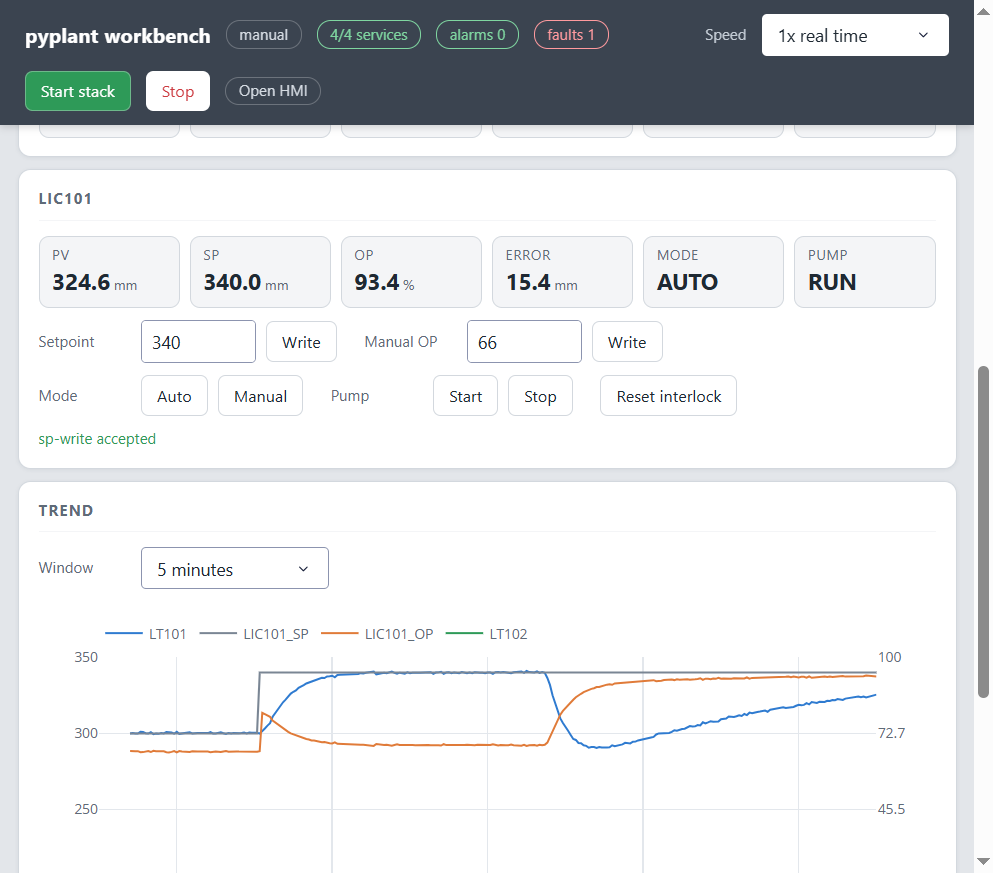
\includegraphics[width=0.62\textwidth]{s09_runtime_leak}}\\[14pt]
\end{center}

\begin{tcolorbox}[colback=panelgrey,colframe=slate,title=The scenario in this guide,
  fonttitle=\bfseries,sharp corners]
Unit~1 (two tanks, pump PMP101, valve FCV101, level loop LIC101) runs in
automatic. We step the level setpoint from 300 to 340\,mm, open a
\textbf{leak in tank~1}, watch the controller hide it, confirm it on the
operator HMI, and then generate data and train four detectors to catch it.
\end{tcolorbox}

\begin{center}
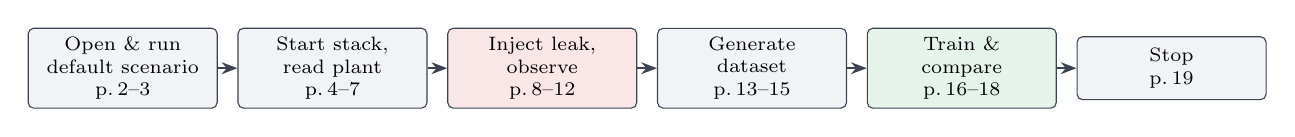
\begin{tikzpicture}[node distance=2.5mm,
  s/.style={draw=slate,fill=panelgrey,rounded corners=2pt,font=\scriptsize,
    align=center,minimum width=24mm,minimum height=8mm},
  >={Stealth[length=2mm]}]
  \node[s] (a) {Open \& run\\default scenario\\p.\,2--3};
  \node[s,right=of a] (b) {Start stack,\\read plant\\p.\,4--7};
  \node[s,right=of b,fill=badred!12] (c) {Inject leak,\\observe\\p.\,8--12};
  \node[s,right=of c] (d) {Generate\\dataset\\p.\,13--15};
  \node[s,right=of d,fill=okgreen!12] (e) {Train \&\\compare\\p.\,16--18};
  \node[s,right=of e] (f) {Stop\\p.\,19};
  \foreach \x/\y in {a/b,b/c,c/d,d/e,e/f} \draw[->,thick,slate] (\x) -- (\y);
\end{tikzpicture}
\end{center}

\noindent\textbf{Start the workbench:}
\begin{center}
\code{conda activate pyplant}\\
\code{python -m pyplant.workbench.app --workspace ./work/manual}
\end{center}
\noindent then open \url{http://127.0.0.1:8050} in a browser.

% --------------------------------------------------------------------- 2
\step{Step 0 -- The workbench at a glance}
{Open \url{http://127.0.0.1:8050}. Nothing is running yet.}
{0.74}{s00_open}{
\item \ui{manual} -- workspace name; all files go to \code{work/manual}.
\item \ui{0/4 services} -- red until plant, PLC, historian and HMI are all up.
\item \ui{alarms} / \ui{faults} -- live counts (``--'' while stopped).
\item \ui{Speed} -- 1$\times$ to 20$\times$ real time, applied at the next start.
\item \ui{Start stack} / \ui{Stop} / \ui{Open HMI} -- control the live services.
\item Tabs \ui{Quick start}, \ui{Runtime}, \ui{Faults}, \ui{Data}, \ui{Model}.
\item Workflow cards 1--5 -- the recommended order; \ui{Go to \ldots} jumps to a tab.
}

% --------------------------------------------------------------------- 3
\step{Step 1 -- Run the default scenario (offline)}
{Scroll to \ui{Default scenario}, keep \ui{Leak in tank 1}, \ui{30 minutes}, press \ui{Run scenario}.}
{0.72}{s01_scenario}{
\item \ui{Scenario} and \ui{Length} dropdowns; \ui{setpoint moves} adds setpoint steps.
\item \ui{Run scenario} -- simulates 30 min of plant time in seconds, no services needed.
\item \ui{LT101 CHANGE +0.02 mm} -- the level hardly moves: the loop hides the leak.
\item \ui{CONTROLLER OP CHANGE +9.64\%} -- the valve opens more: this is the fault signature.
\item \ui{PUMP TRIP none}, \ui{FAULT ONSET 720 s}.
\item Chart -- levels on the left axis, OP and valve position on the right; red band = fault.
}

% --------------------------------------------------------------------- 4
\step{Step 2 -- Runtime tab before starting}
{Click the \ui{Runtime} tab.}
{0.74}{s02_runtime_stopped}{
\item \ui{SERVICES} -- one row per service with \ui{STATE}, \ui{PID}, \ui{PORT}, \ui{ROLE}.
\item Red \ui{down} pills -- nothing is running.
\item \ui{UNIT 1} mimic shows ``--'' until the PLC answers.
}

% --------------------------------------------------------------------- 5
\step{Step 3 -- Start the stack}
{Keep \ui{Speed} at \ui{1x real time} and press \ui{Start stack}.}
{0.74}{s03_runtime_services}{
\item \ui{stack started at 1x} -- confirmation under the header.
\item \ui{4/4 services} badge turns green; \ui{alarms 0}, \ui{faults 0}.
\item Every service \ui{up}, with its PID and port (plant 5400, plc 5402, historian 5404, hmi 5405).
\item Grey line -- the exact command line used, handy for running a service by hand.
}

% --------------------------------------------------------------------- 6
\step{Step 4 -- Read the healthy plant}
{Scroll to \ui{UNIT 1}. Remember these values as the healthy reference.}
{0.74}{s04_runtime_mimic}{
\item \ui{PMP101} pump (green = running) and \ui{FCV101} valve at 66.1\,\%.
\item \ui{TANK 1} 300.0\,mm (LT101) and \ui{TANK 2} 176.8\,mm (LT102).
\item Flow tiles \ui{FT101} 10.08 and \ui{FT102} 10.05\,L/min -- in balance.
\item \ui{PT101} pump pressure, \ui{ZT101} valve position.
\item \ui{SCAN} 3.70\,ms of a 100\,ms budget; \ui{OVERRUNS} must stay 0.
}

% --------------------------------------------------------------------- 7
\step{Step 5 -- Operate LIC101: setpoint step}
{Type \code{340} in \ui{Setpoint}, press its \ui{Write}, wait about 2 minutes.}
{0.72}{s05_faceplate_trend}{
\item \ui{PV} / \ui{SP} / \ui{OP} / \ui{ERROR} -- 339.7\,mm, 340.0\,mm, 68.6\,\%, 0.3\,mm.
\item \ui{MODE AUTO}, \ui{PUMP RUN}.
\item \ui{Setpoint}+\ui{Write}, \ui{Manual OP}+\ui{Write} (used in Manual mode only).
\item \ui{Auto} / \ui{Manual}, pump \ui{Start} / \ui{Stop}, \ui{Reset interlock}.
\item \ui{sp-write accepted} -- the PLC took the new setpoint.
\item \ui{TREND} -- clean step: level rises to 340\,mm with no overshoot.
}

% --------------------------------------------------------------------- 8
\step{Step 6 -- The Faults tab}
{Click the \ui{Faults} tab.}
{0.72}{s06_faults_empty}{
\item \ui{BREAK SOMETHING} -- one-click presets (leak, slow leak, sticking valve, worn pump, fouling, sensor faults).
\item \ui{Clear all faults} -- removes every active fault.
\item \ui{OR BUILD ONE} -- \ui{Kind}, \ui{Magnitude} ($-$/$+$, unit shown on the right), \ui{Sensor}, \ui{Ramp (s)}.
\item \ui{Inject} -- applies the custom fault.
\item \ui{ACTIVE FAULTS} -- ``Plant is healthy.''
}

% --------------------------------------------------------------------- 9
\step{Step 7 -- Inject the leak}
{Press \ui{Leak in tank 1}.}
{0.72}{s07_fault_injected}{
\item \ui{faults 1} -- the header badge turns red.
\item Message: \ui{injected leak\_168 on TANK1 -- watch the Runtime tab}.
\item \ui{ACTIVE FAULTS} row: leak\_168, leak, TANK1, \ui{active}, 0.000050\,m$^2$, start 169\,s, ramp 0.
}
\tip{Neither the HMI nor any model is told about the fault -- you find it by watching the plant.}

% --------------------------------------------------------------------- 10
\step{Step 8 -- Ground truth vs.\ instruments}
{Scroll down to \ui{Ground truth against what the instruments report}.}
{0.72}{s08_truth}{
\item \ui{TRUE} -- the real value inside the simulator.
\item \ui{REPORTED} -- what the transmitter sends.
\item \ui{DIFFERENCE} -- all within noise ($<$0.3): it is a \emph{process} fault, not a sensor fault.
\item The true level, 299.3\,mm, is already 40\,mm under the setpoint.
}

% --------------------------------------------------------------------- 11
\step{Step 9 -- Watch the controller fight the leak}
{Back to \ui{Runtime}, scroll to \ui{LIC101}, about 2 minutes after injection.}
{0.72}{s09_runtime_leak}{
\item \ui{PV 324.6 mm}, \ui{ERROR 15.4 mm} -- recovering, slowly.
\item \ui{OP 93.4\,\%} -- up from 68.6\,\%: the valve is nearly wide open.
\item No alarm, no trip: \ui{AUTO}, \ui{RUN}.
\item Trend: first the setpoint step, then the leak -- level dips to $\approx$290\,mm, OP jumps and stays high.
}

% --------------------------------------------------------------------- 12
\step{Step 10 -- The operator HMI}
{Click \ui{Open HMI} (or open \url{http://127.0.0.1:5405}).}
{0.72}{s10_hmi}{
\item Header: \ui{connected} (OPC UA live), \ui{alarms 0}, \ui{AUTO}, PLC time.
\item \ui{MIMIC} in dark style; tank~1 328.4\,mm, tank~2 188.4\,mm.
\item \ui{FT101 18.30 L/min} (was 10), \ui{PT101 27.9 kPa} (was 50), \ui{ZT101 93.4\,\%}.
\item \ui{LIC101} panel -- same controls as the workbench faceplate.
\item \ui{TREND} with \ui{Window} 2\,min--1\,h; \ui{ALARMS} with \ui{Acknowledge all} below.
}
\tip{The level never crossed an alarm limit. Only the extra 8\,L/min of inflow and a wide-open valve give the leak away.}

% --------------------------------------------------------------------- 13
\step{Step 11 -- Clear the fault, open the Data tab}
{On \ui{Faults} press \ui{Clear all faults}, then click \ui{Data}.}
{0.72}{s11_data_form}{
\item \ui{faults 0} -- the plant is healthy again.
\item \ui{Preset} -- \ui{Quick} ($\sim$1.5\,min), \ui{Standard} ($\sim$4\,min), \ui{Thorough} ($\sim$10\,min).
\item \ui{Run length}, \ui{Magnitudes}, \ui{Repeats}, \ui{Normal runs}.
\item \ui{Generate} / \ui{Cancel}, and the progress bar under them.
\item \ui{RECENT RUNS} -- job history (kind, status, took, result).
}

% --------------------------------------------------------------------- 14
\step{Step 12 -- Generate a Quick dataset}
{Press \ui{Quick (\textasciitilde1.5 min)}, then \ui{Generate}.}
{0.72}{s12_data_running}{
\item Fields change to 1200\,s, 1 magnitude, 1 repeat, 6 normal runs.
\item \ui{started} and the bar filling blue.
\item \ui{dataset -- running -- 17 s} in \ui{RECENT RUNS}.
}
\tip{Data generation uses the offline fast runner in its own process; the live plant keeps running untouched.}

% --------------------------------------------------------------------- 15
\step{Step 13 -- Dataset ready}
{Wait until the bar is full (about 45\,s).}
{0.72}{s13_data_done}{
\item Full bar -- job finished.
\item \ui{dataset -- ok -- 43 s}.
\item Result: 14 runs (6 normal + 8 faulty), 16\,814 samples,\\
  saved as \code{work/manual/dataset.parquet} (1.7\,MB).
}

% --------------------------------------------------------------------- 16
\step{Step 14 -- Set up training}
{Click the \ui{Model} tab.}
{0.72}{s14_model_form}{
\item \ui{Methods} -- Z-score limits, PCA/MSPC, Isolation forest, Autoencoder (all ticked).
\item \ui{Window} 60 samples, \ui{Stride} 10.
\item \ui{Quantile} 0.995 -- alarm threshold on normal data; higher = fewer false alarms, later detection.
\item \ui{Train} -- starts the training job.
\item \ui{RESULTS} -- ``no model trained yet''.
}

% --------------------------------------------------------------------- 17
\step{Step 15 -- Train and compare}
{Press \ui{Train}. About 12\,s on the Quick dataset.}
{0.72}{s15_model_results}{
\item \ui{detected} -- z-score 62\,\%, \textbf{PCA 88\,\%}, isolation forest 38\,\%, autoencoder 88\,\%.
\item \ui{median delay} -- 43\,s for PCA and autoencoder.
\item \ui{false alarms/day} -- 0.00 for all.
\item \ui{pca (selected)} -- tie with the autoencoder, so the simpler method is deployed.
}
\tip{If the table still says ``no model trained yet'' after the job ends, reload the page.}

% --------------------------------------------------------------------- 18
\step{Step 16 -- Results per fault mode}
{Scroll to \ui{BY FAULT MODE}.}
{0.72}{s16_by_mode}{
\item One row per fault mode: \ui{runs}, \ui{detected}, \ui{median delay}.
\item \textbf{leak}: 2 runs, 100\,\% detected, 139\,s after onset.
\item \ui{top channel} = \ui{expected} = FLOW\_IMBALANCE -- the leak is also correctly isolated.
\item \ui{not scored} -- sensor faults, where isolation does not apply.
}

% --------------------------------------------------------------------- 19
\step{Step 17 -- Stop the stack}
{Press \ui{Stop} in the header.}
{0.72}{s17_stopped}{
\item \ui{stack stopped}, \ui{0/4 services}, all rows \ui{down}.
\item Results stay in \code{work/manual}:
  \code{config.json}, \code{history.duckdb}, \code{dataset.parquet},\\
  \code{artifacts/detector.joblib} and \code{artifacts/metrics.json}.
}

% --------------------------------------------------------------------- 20
\clearpage
\begin{tcolorbox}[colback=slate,colframe=slate,coltext=white,sharp corners,boxsep=3pt,left=6pt]
\large\bfseries Cheat sheet
\end{tcolorbox}

\begin{center}
\fcolorbox{slate!40}{white}{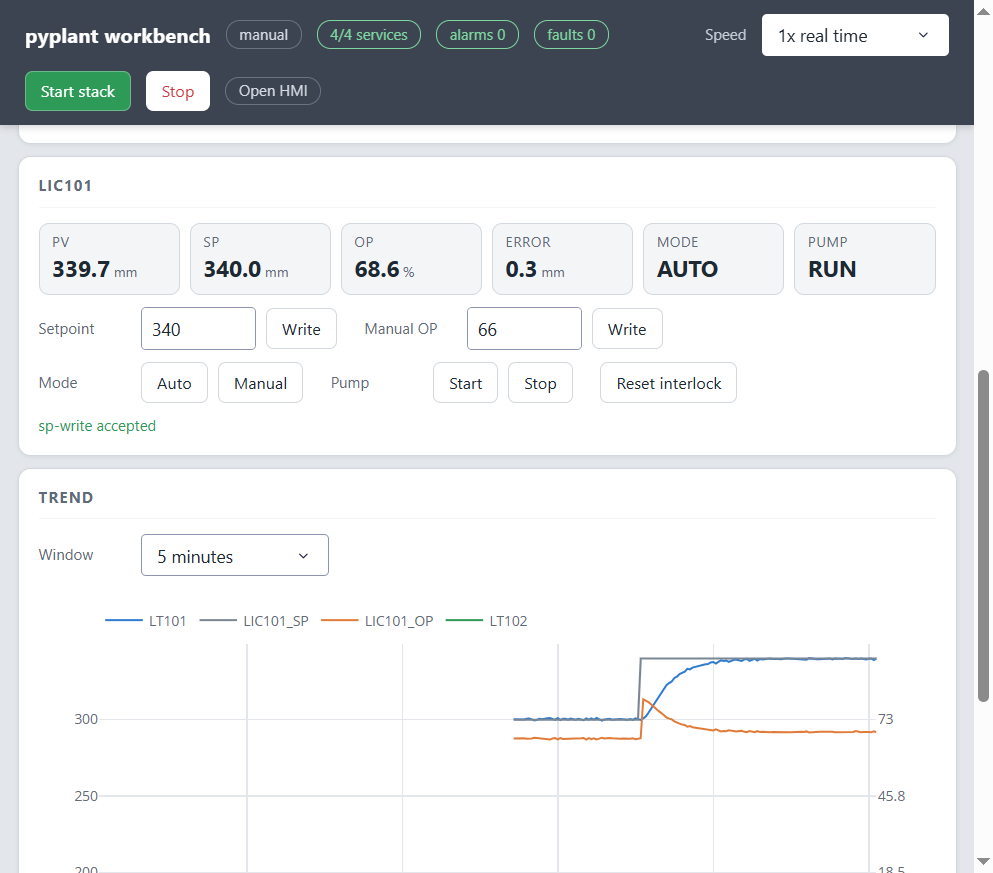
\includegraphics[width=0.42\textwidth]{s05_faceplate_trend}}\hspace{4mm}%
\fcolorbox{slate!40}{white}{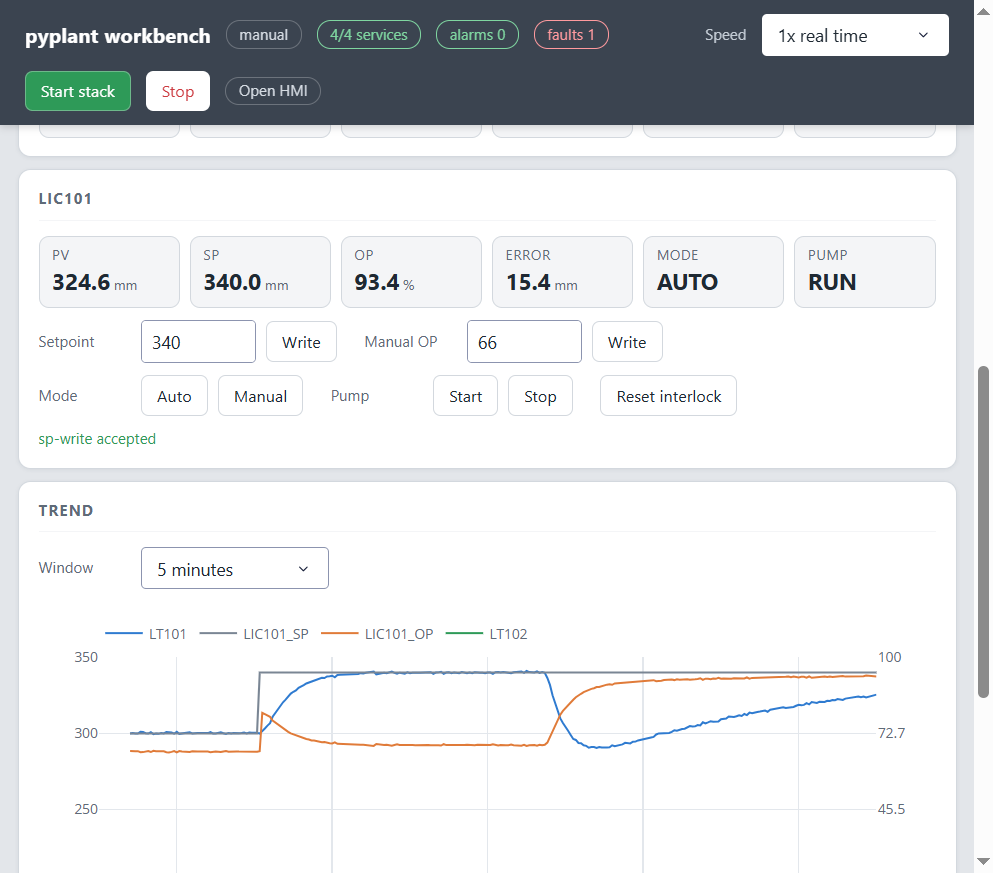
\includegraphics[width=0.42\textwidth]{s09_runtime_leak}}\\[2pt]
{\small Healthy setpoint step (left) vs.\ leak (right): a process fault moves \textbf{OP}, not the level.}
\end{center}

\begin{tcolorbox}[colback=panelgrey,colframe=slate,title=Where things are,fonttitle=\bfseries,sharp corners]
\small
\begin{tabular}{@{}p{0.3\linewidth}p{0.62\linewidth}@{}}
Workbench & \url{http://127.0.0.1:8050} \\
Operator HMI & \url{http://127.0.0.1:5405} (button \ui{Open HMI}) \\
Ports & plant 5400, PLC 5402, OPC UA 5403, historian 5404, HMI 5405 \\
Workspace & \code{--workspace ./work/<name>}; all data, models and logs inside \\
Service logs & \code{work/<name>/jobs/*.log}
\end{tabular}
\end{tcolorbox}

\begin{tcolorbox}[colback=accent!5,colframe=accent,title=Fault signatures,fonttitle=\bfseries,sharp corners]
\small
\begin{tabular}{@{}p{0.3\linewidth}p{0.62\linewidth}@{}}
Leak & OP and FT101 rise, level dips then recovers, ground truth agrees \\
Sticking valve & ZT101 lags OP in steps, level cycles \\
Worn pump & PT101 and FT101 drop at the same OP \\
Fouled interconnect & LT101 rises relative to LT102, FT102 falls \\
Sensor bias / frozen & ground-truth DIFFERENCE for that tag is large
\end{tabular}
\end{tcolorbox}

\begin{tcolorbox}[colback=okgreen!5,colframe=okgreen!70!black,title=If something goes wrong,fonttitle=\bfseries,sharp corners]
\small
\begin{itemize}
\item \ui{0/4 services} after start -- a port is busy; stop old runs or change \code{--base-port}.
\item \ui{OVERRUNS} counting up -- lower the \ui{Speed}.
\item Pump tripped -- raise the level (Manual OP), then \ui{Reset interlock} and \ui{Start}.
\item Panels stop updating -- reload the page; jobs keep running in the background.
\item ``generate a dataset first'' on \ui{Train} -- run step 12 before step 15.
\end{itemize}
\end{tcolorbox}

\end{document}
